\documentclass{article}

\usepackage{graphicx} % Required for inserting images
\usepackage{amsthm}
\usepackage{amssymb}
\usepackage{titlesec}
\usepackage{blindtext}
\usepackage{mathtools}
\usepackage{listings}


\setcounter{secnumdepth}{0}

\title{Finding Dimensions Of Spanning Vectors And Other Problems In Linear Algebra}
\author{Ben Lowe, Caleb Loveridge, Rebecca Grimshaw, Chloe Godwin, Moritz Hartmann }
\date{October 2023}

\begin{document}

\maketitle

\tableofcontents

\break


\section{Part A Question 1}
A field is a set of elements which satisfy the distributively of multiplication over a vector and distributively of vectors over a field of scalars. They must also satisfy the property that the multiplicative identity on the fields also acts as a multiplicative identity over the vector space. Finally we have associativity of the scalars over the vector field, that is to say $\alpha (\beta \bar{V} )= (\alpha \beta ) \bar{V} $.

Vector spaces unlike fields don't have a multiplicative binary operation. And, unlike the vector space a field doesn't have some binary operation with some other space.

\subsection*{Part A Question 2}

We find the applications of mathematics to our specific areas of interest. For example, finding areas of physics which uses abstract algebra like the beauty of group theories application in Noethers Theorem or applications in probability such using probability distributions to forecast business outcomes resulting from various possible decisions. 

\subsection*{Part A Question 3}
The transformation between 3D Cartesian coordinates is non-linear for example the distance between points decreases as you go north or south along a line of longitude from the equator. This is because the surface of the earth is non-Euclidean, parallel lines may converge at the poles. 

\subsection*{Part A Question 4}
We've are proactive at organising a meeting allowing us to finish the project in ample time to review and improve our answers. We've been using technology effectively to facilitate communication between members of the group allowing us to work better as a team. We all arrived on time to our meetings showing that we are enthusiastic to complete the tasks assigned to us. We also have been distributing the tasks clearly and equitably to produce better outcomes and to ensure that all tasks are completed on time. We sit together in lectures so that we're better able to learn and develop together and better understand the linear algebra concepts. We're comfortable with asking each other for help when we don't understand something and have a group who is ready and able to help each other for example we struggled to understand the dimension of the complex vector space in the reals so we were able to work together and find an answer to question 1 part A.

\break

\section{Part B Question 1}

\subsection{Part B Question 2}
We are given the matrices.

\begin{equation*}
    A  \coloneqq \begin{bmatrix}
        1 & 2\\3&4 
    \end{bmatrix}
\end{equation*}
\begin{equation*}
    \overline{x}  \coloneqq \begin{bmatrix}
        3 \\ 2
    \end{bmatrix}
\end{equation*}
\begin{equation*}
    \overline{y} \ \coloneqq \begin{bmatrix}
        -1 \\ 5
    \end{bmatrix} 
\end{equation*}

We can then evaluate $<\bar{a}|\bar{B}> \vcentcolon \coloneqq \Bar{a}^TA\bar{y}$ for the four combinations in the equasion.

\begin{equation*}
    <\overline{x}|\overline{y}>_A = \begin{bmatrix}
        3 & 2
    \end{bmatrix}
    \begin{bmatrix}
        1&2\\3&4
    \end{bmatrix}
    \begin{bmatrix}
        3\\2
    \end{bmatrix}
    =
    \begin{bmatrix}
        3 & 2
    \end{bmatrix}
    \begin{bmatrix}
        7\\17
    \end{bmatrix}
    = 55
\end{equation*}
\begin{equation*}
    <\bar{x}|\bar{y}>_A = \begin{bmatrix}
        3 & 2
    \end{bmatrix}
    \begin{bmatrix}
        1&2\\3&4
    \end{bmatrix}
    \begin{bmatrix}
        -1\\5
    \end{bmatrix}
    =
    \begin{bmatrix}
        3 & 2
    \end{bmatrix}
    \begin{bmatrix}
        9\\17
    \end{bmatrix}
    = 61
\end{equation*}
\begin{equation*}
    <\bar{x}|\bar{y}>_A = \begin{bmatrix}
        -1 & 5
    \end{bmatrix}
    \begin{bmatrix}
        1&2\\3&4
    \end{bmatrix}
    \begin{bmatrix}
        3\\2
    \end{bmatrix}
    =
    \begin{bmatrix}
        -1 & 5
    \end{bmatrix}
    \begin{bmatrix}
        7\\17
    \end{bmatrix}
    = 78
\end{equation*}
\begin{equation*}
    <\bar{x}|\bar{y}>_A = \begin{bmatrix}
        -1 & 5
    \end{bmatrix}
    \begin{bmatrix}
        1&2\\3&4
    \end{bmatrix}
    \begin{bmatrix}
        -1\\5
    \end{bmatrix}
    =
    \begin{bmatrix}
        -1 & 5
    \end{bmatrix}
    \begin{bmatrix}
        9\\17
    \end{bmatrix}
    = 76
\end{equation*}

Then for the second part of the questions we have the bilinear form $<(1,0,0)|(1,0,0)>_A = 1$,$<(0,1,0)(0,0,1)>_A = 5$ and $<(0,0,1)(0,0,1)_A = 3$. We then need to find the $3$ by $3$ matrix which is given by the bilinear form A containing terms $a_{i,j}$ with $i,j \in \{ 1,2,3\}$.

From the first equasion we see that $a_{1,1} = 1$ so that the product of the two first elements of our vectors are $1$. Similarly, we get that $a_{3,2} = 5$ as the third and second elements of the vectors must be equal to 5, all other elements go to zero. Finally, we must evaluate the last equasion with $a_{1,3}, a_{2,3}, a_{3,3}$ as free variables because the third element is the only none zero element of RHS vector. We can then solve for the three variables as $3 = a_{1,3} + a_{2,3} - 2 a_{3,3}$, And so we can choose the values for example $a_{1,3} = 1, a_{2,3} = 2, a_{3,3} = 3$ which then give us the Matrix $A$.

\begin{equation*}
    A = \begin{bmatrix}
        1&0&0 \\ 0 & 0 & 5 \\ 3 & 2 & 1
    \end{bmatrix}
\end{equation*}

\subsection{Part B Question 3}
 For question 1.70(iii) we have that $B = (1+x,1-x,x + x^2) \in P_2(\mathbb{C}$. This means $1+x \implies (1,1,0)$, $1-x \implies (1,-1,0)$, $1+x \implies (0,1,1)$

We want to find $\alpha_1, \alpha_2, \alpha_3 \in \mathbb{R}$ such that $\alpha_1 (1,1,0) + \alpha_2(1-x) +\alpha_3 (x + x^2) = 1 + x - x^2$ or similarly.

\begin{equation}
    \begin{bmatrix}
        1 & 1 & 0 \\ 1& -1& 1 \\ 0 &0 &1
    \end{bmatrix}
    \begin{bmatrix}
        \alpha_1 \\ \alpha_2 \\ \alpha_3
    \end{bmatrix}
    =
    \begin{bmatrix}
        1 &1& -1
    \end{bmatrix}
\end{equation}

This implies $\alpha_1 + \alpha_2 = 1$, $\alpha_1 - \alpha_2 + \alpha_3 = 1$, $\alpha_3 = -1$ which then implies $\alpha_1 = 1- \alpha_2$. 
We then substitute this into the second equasion and solve for $\alpha_2$ finding $\alpha_1 = 1-\alpha_2$ so $1-2\alpha_2 = 1-\alpha_3$. 
Then since we know $\alpha_3 = -1$ we have that $1-2\alpha_2 = 2$ so $\alpha_2 = 1\frac{1}{2}$. This then means $\alpha_1 = 1- \frac{-11}{2} = \frac{3}{2}$. So we find.

\begin{equation}
    \begin{bmatrix}
        1 + x -x^2
    \end{bmatrix}_B
    =
    \begin{bmatrix}
        \frac{3}{2} & -\frac{1}{2} & -1
    \end{bmatrix}
\end{equation}

Then for question 11.76 we let $A,B,C \in M_2(\mathbb{R})$ and $\alpha_1, \alpha_2 \in \mathbb{R}$. If the statement is true then we should end up with $A = \alpha_1B +\alpha_2 C$. So, we write $B = \frac{A + A^T}{2}$. Then we evaluate the matrix $B^T = \frac{(A+A^T)^T}{2} = frac{ A^T + A}{2} = B$. Therefore we know that B is a symmetric matrix. 

We can next consider $C = \frac{(A-A^T)}{2}$ and then evaulate $C^T = \frac{(A-A^T)^T}{2} = \frac{-(A^T - A)}{2} = \frac{-(A-A^T)}{2} = -C$. Therefore we see that $C$ is skew symmetric. 

Next, we consider $B+C = \frac{A + A^T}{2} + \frac{(A-A^T)}{2} = \frac{A+A^T+A-A^T}{2} = \frac{2A}{2} = A$.

Since we can write $A = B+C$ where $\alpha_1, \alpha_2 = 1$, it is possible to write any matrix $A \in M_2(\mathbb{R})$ as linear combinations of symmetric and skew symmetric matrices.


\subsection{Part B Question 4}
For exercise 1.81 let V be the subspace of functions $f: \mathbb{R} \rightarrow \mathbb{R}$. To show whether the following are subspaces of V we have to check if the subspace axioms are satisfied:

S1. $\mathbf{0} \in V$

S2. If $\bold{v}, \bold{w} \in V$ then $\bold{v} + \bold{w} \in V$

S3. if $\alpha \in F$ and $\bold {v} \in V$ then $\alpha \bold{v} \in V$

For part i we have that the zero vector is $f: \mathbb{R} \rightarrow \mathbb{R}$, such that all the coefficients are zero. And, thus maps every $x \in \mathbb{R} \rightarrow 0$. This gives $\bold{0} \equiv 0 e^x + 0e^{-x} + 0 ; a,b,c = 0 \in \mathbb{R}$. 

Graphically, this is shown in Figure 1.

\begin{figure}[ht]
    \centering
    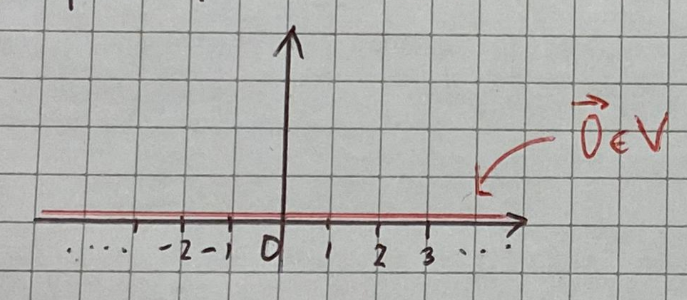
\includegraphics[scale = 0.6]{Figure.png}
    \caption{Graph of $\bold{0}$}
    \label{fig:enter-label}
\end{figure}

For part ii we let $T = \{ f\in V | f(0) = 2 \}$ and check the conditions for a subspace S1 we find that $\bold{0} \notin V$ because $f(0) = 2$ whereas $\bold{0}(0) = 0$ so S1 doesn't hold. Therefore T is not a subspace of V.

Finally, for part iii we let $S = \{ f \in V | f(x) = a(e^x - e^{-x}), a \in \mathbb{R} \} $. Checking the conditions for a subspace we check:

S1 $\bold{0} \in S $ since $0 \cdot (e^x - e^{-x}) - 0, \forall x \in \mathbb{R}$.

S2 We let $b(e^x - e^{-x})$ and $c(e^x - e^{-x})$ both be in S where $b,c \in \mathbb{R}$. Then we consider $b(e^x - e^{-x}) + c(e^x - e^{-x}) = (b+c)e^x - e^{-x})$ where $(b+c) \in \mathbb{R}$ as the field is closed so the sum is in S for all $b,c \in \mathbb{R}$.

S3 Let $\alpha \in \mathbb{R}$ and $a (e^x - e^{-x}) \in S$ then $\alpha a \in \mathbb{R}$ so $\alpha a (e^x - e^{-x}) \in S$.




\subsection{Part B Question 5 }
This line declares the "sequence of n vectors" included in the theorem to be proven, so they then must show that this forms a basis. Specifically a basis of a subspace of the set V. However, the student is yet to specify if the span of the sequence of vectors is equal to V or not, this may be answered later in the proof.

The student is asserting that $dim(V) = n$ where $n$ is also the cardinality of the sequence of vectors mentioned on the first line. Since, we know that $(w_1,...,w_n)$ are independent and minimal from the assertion that $dim(V) = n$ if 1.58 is true we would get that $(W_1,...,w_n)$ is a basis. So, maybe the student is now going to show that it is implied that this is a basis.

The next clause uses the fact that $V$ is finite dimensional from the last clause to show that the minimal spanning set of $V$ is finite due the the definition of dimension.

We now see that if W is a spanning set of the sequence of vectors which would mean that if $V$ was equal to $W$ then the sequence of vectors must also be a spanning set of $V$.

The student goes on to explain this idea of $V=W$ showing that the sequence of vectors is a basis; adding that this is due to it satisfying the definition of a basis as $w_i$ spans V. The student would also need to show that the span is minimal which the student hasn't mentioned explicitly but can be gained from knowing $dim(V) = n$.

The student is proving this part by contradiction so assuming that $V \neq W$ then showing this implies either the $w_i$ sequence is not linearly independent or maybe showing some other contradiction with the assertions the student has already made like $dim(V) \neq n$.

The student says that there must be a $v_i \notin W$. 
This is by the definition for two sets to be equal, that for all $v_i \in W \Rightarrow v_i \in V$ and 
$v_i \in V \Rightarrow v_i \in W$ 
so its negation $V \neq W$ would mean there exists some $v$ which doesn't satisfy either of the statements. 

Theorem 1.40 then tells us that for subspaces $W \subset V$ and v is spanned by n vectors then $r\leq n$ where $r$ is the basis aka linearly independent sequence of $W$. For our case this would mean that since 
$dim(V) = n$ we can add another linearly independent vector to the span of $w$ from $v$ knowing they're linearly independent as 
$v_i \notin W$.

We then count the span of linearly independent vectors we've found and see that the sequence has $n+1$ independent vectors that span the space. However theorem 1.44 will tell us that the linearly independent sequence of vectors we found $(w_1,...,w_n,v_i)$ which spans the space must therefore be a basis of $V$. This then means that $dim(V) = n+1$ by the definition of dimension as being the cardinality of the basis. This is a contradiction as we already know that $dim(V) = n$. we can therefore see that $V=W$ so then n vectors must be both minimal and spanning hence the n vectors form a basis by theorem 1.44.

The problem with this proof comes from the use of theorem 1.40 which applies to spaces $W \subset V$ however we otherwise might have that $V \subset W$ then $W\neq V$ still holds. Further, the part of the theorem $r \leq n$ is not strictly less than so we could have that $r = n$ even if $W\neq V$ as just because the dimensions are the same then the sets don't have to be. This means that $v_i$ might not be linearly independent with $(w_1,...w_n)$.

\break

\section{Part C}
We have two methods for computing the dimension of the space. For both methods we use a row space representation of the spanning vectors then we know that the rank of the matrix is therefore the dimension of the row space\cite{Johnson}.
The first of these methods is finding the rank explicitly by computing the reduced row echelon form of the matrix, this also gives a basis of the space\footnote{Theorem 1.47}. 
The other method uses the minor method to find all the minor sub-matrices of the row space matrix, and if the determinant is none zero we know those rows are independent\footnote{Corollary 1.59}, we can then use this fact about independence to find the dimension\footnote{Theorem 1.58}.
\subsection*{Row Reduced Echelon Form}
We first put the spanning vectors into a row space matrix then row reduce them. We do this using the Gauss-Jordan method\cite{Dobrushkin}. First, we order the rows in decreasing pivot position and magnitude. Next, we can subtract the nth row from those below it so that no pivots share a column with another number. Finally, we divide the pivots by themselves to make sure they're all equal to zero. Note, other sources\cite{CueMath} use alternate but equivalent Gauss-Jordan methods.

\subsection*{Minor Method}
For the minor method we test if each of subsets of rows are independent using the determinant test\footnote{Corollary 1.59} then we can count the number of independent rows to find the dimension\cite{CueMath}. The determinant was calculated using Laplace expansion\cite{CliffsNotes}\cite{OpenAI}. 

\subsection*{r,n and d Relationship}
We found that for $r$ spanning vectors of a subspace of $\mathbb{R}^n$ has a dimension d. We know that $d \leq n$\footnote{Corollary 1.61}. We also find that when computing the row reduction of a matrix the none zero rows can only decrease which means that $d\leq r$.

\subsection*{Expected Dimension}
We also investigated the expected dimension for $r$ random spanning vectors in $\mathbb{R}^n$ using a function to trial $100,000$ different sequences of vectors we found that the expectation for $d$ the dimension of the subspace is $d = min(r,n)$. 

\break

\begin{thebibliography}{11}

\bibitem{Johnson}
Johnson, J,. (2000)
https://web.math.princeton.edu/$\sim$jmjohnso/teaching/202Bfall00/

\bibitem{Shao}
Shao, Y,. 
https://www.math.purdue.edu/\~shao92/documents/Algorithm\%20REF.pdf and 

\bibitem{Dobrushkin}
Dobrushkin, V,. https://www.cfm.brown.edu/people/dobrush/cs52/Mathematica/Part1/rref.html

\bibitem{CueMath}
CueMath. https://www.cuemath.com/algebra/rank-of-a-matrix/

\bibitem{CliffsNotes}
Cliffs Notes. https://www.cliffsnotes.com/study-guides/algebra/linear-algebra/the-determinant/laplace-expansions-for-the-determinant

\bibitem{OpenAI}
OpenAI. (2022). GPT-3.5. https://chat.openai.com/

\end{thebibliography}

\break

\section{Appendix}

Python files are available at: https://github.com/BenLowe2003/MATH220\_Project001\_Dimensionality

\begin{lstlisting}[language=Python, caption=Functions In Linear Algebra, label=fuctions]
#We define a function to perform the swap elementry row 
operation
def row_swap(M,p,q):
    #Determine the size of the matrix so we dont need to 
    have extra arguments in the function.
    n = len(M)
    m = len(M[0])
    #Create a variable to store the row which is going to 
    be replaced
    temp = M[p]
    #replace the row p with row q
    M[p] = M[q]
    #replace row q with the copy of row p
    M[q] = temp
    return M

#We define a function to perform addition elementry row 
operation.
def row_addition(M, p, q, f):
    #Temporarily store the rows p and q for saftey
    tempq = M[q]
    tempp = M[p]
    
    #iterate through the row performing the operation to 
    each of the elements in row p
    for i in range(len(tempp)):
        tempp[i] = tempp[i] + f * tempq[i]
    # return the temporary row variables in the matrix
    M[p] = tempp
    M[q] = tempq
    return M

#We define a function to perform scaler multiplication 
elementry row operation.
def row_multiplication(M, p, f):
    #Temporarily store row p for saftey
    temprow = M[p]
    #Iterate through row p multiplying each element by f
    for i in range(len(temprow)):
        temprow[i] = f*temprow[i]
    #return the temporary row into the matrix
    M[p] = temprow
    return M

#We define a function to put all teh zero rows at teh end 
of a matrix using row reduction.
def organise_zero_rows(M):
    #We determine the dimensions of M
    num_rows = len(M)
    num_columns = len(M[0])
    #Create a list of all the zero rows
    zero_rows = []
    #we then iterate through the rows to check fi they're 
    zero rows.
    for i in range(num_rows):
        #create a boolean to see if this row is a zero row
        is_zero_row = True
        #iterate through each row check if each element in 
        row i is 0.
        for j in range(num_columns):
            #check if the element is not zero
            if M[i][j] != 0:
                #if the element is not zero we know its 
                not a zero row.
                is_zero_row = False
        #check if its definatly a zero row
        if is_zero_row == True :
            #if its a zero row add it to the list of zero 
            rows
            zero_rows.append(i)
    #we find out how many zero rows we have so that we 
    know where to put them
    num_zero_rows = len(zero_rows)
    #we find out where to put the first zero row
    place_row_index = num_rows - num_zero_rows
    #we then iterate through the zero rows putting them at 
    the bottom of the matrix
    for i in zero_rows:
        #if its a zero row we swap it with one of the
        row_swap(M, i, place_row_index)
        #we then find the index of our next row
        place_row_index -= 1
    return M

#we define a function to put the largest pivot points at 
the top.
def organise_pivots(M):
    #We determine the dimensions of M
    num_rows = len(M)
    num_columns = len(M[0])
    #We then do a bubble sort cause its easiest to 
    implement.
    #Create a boolean to check if its sorted.
    sorted_check = False
    #We repeat the bubble sort until the list is sorted
    while sorted_check == False:
        #set soted check to true until we find ut where 
        its not sorted.
        sorted_check = True
        #We iterate through the columns to swap neighbours
        for i in range(num_rows - 1):
            # we find which of the ith and i+1th element 
            is none zero and and laregst.
            for j in range(num_columns):
                #check if we need to swap them.
                if (M[i][j] < M[i+1][j]):
                    #if row i+1 is bigger than i the we 
                    swap so the biggest is on top with the 
                    smallest index
                    row_swap(M,i,i+1)
                    sorted_check = False
                #We then check if we've searched 
                sufficiently through this row.
                if M[i][j] != 0 or M[i+1][j] != 0:
                    #we move onto the next bubble
                    break
    return M

#We next define a function to make all the elements below 
each pivot are zero.
def row_eschelon(M):
    #We determine the dimensions of M
    num_rows = len(M)
    num_columns = len(M[0])
    #We then iterate through each of the rows
    for pivot_row in range(num_rows):
        #for each row we iterate through to find the pivot
        for pivot_column in range(num_columns):
            if M[pivot_row][pivot_column] != 0:
                #we evaluate the pivot value and store it 
                in a variable
                pivot_value = M[pivot_row][pivot_column]
                #we iterate though all the rows below 
                doing additons until the elements are all 
                zeros
                for changed_element_row in range(num_rows):
                    #we make sure not to subtract a row by 
                    itself
                    if changed_element_row != pivot_row:
                        multiplier = -
                        M[changed_element_row]
                        [pivot_column]/pivot_value
                        row_addition(M, 
                        changed_element_row, pivot_row, 
                        multiplier)
                break
    return M

#We define a function to make all the pivots equal to 1
def pivot_normalisation(M):
    #We determine the dimensions of M
    num_rows = len(M)
    num_columns = len(M[0])
    #we iterate through all the rows
    for pivot_row in range(num_rows):
        #iterate through the row until we find the pivot
        for pivot_column in range(num_columns):
            #check if we have the pivot
            if M[pivot_row][pivot_column] != 0:
                #we find out what we need to multiply the 
                row by.
                multiplier = 1/M[pivot_row][pivot_column]
                row_multiplication(M, pivot_row, 
                multiplier)
                break
    return M

#we define a function to perform the entire gauss jordan 
operation from the function steps we've already defined
def reduced_row_eschelon(M):
    #We let M equal to its reduced form
    M = pivot_normalisation(row_eschelon(organise_pivots(organise_zero_rows(M))))
    return M
    
#we define a function to take the transverrse of a matrix
def transpose(M):
    #We determine the dimensions of M
    num_rows = len(M)
    num_columns = len(M[0])
    #we initialise a new natrix
    transpose = [[None] * num_rows for _ in 
    range(num_columns)]
    #we iterate through the rows and columns of M
    for row in range(num_rows):
        for column in range(num_columns):
            #we add the element to transverse with 
            opposite row and column indicies
            transpose[column][row] = M[row][column]
    return transpose

#we define a function to take the matrix product of two 
matrices
def matrix_product(N,M):
    #We find the dimensions of our output matrix and the 
    number of terms in each sum
    num_rows = len(N)
    num_columns = len(M[0])
    num_terms = len(M)
    #initialise an ourput matrix
    T = [[None] * num_rows for _ in range(num_columns)]
    #iterate through evaluating the lements of T
    for row in range(num_rows):
        for column in range(num_columns):
            #we initialise a temporary variable to 
            calculate the element
            temp_element = 0
            #We then iterate through all theh terms that 
            make up the element in T
            for term_index in range(num_terms):
                #we add the term to our temporary element
                temp_element += M[term_index][column] * 
                N[row][term_index]
            #pass the sum into the output matrix
            T[row][column] = temp_element
    return T

#we define a function to eliminate the zero row from a 
matrix
def eliminate_zero_rows(M):
    #we find the dimensions of the matrix
    num_rows = len(M)
    num_columns = len(M[0])
    #create a list to store all the none zero rows
    none_zero_rows = []
    #we iterate through all the rows
    for row in range(num_rows) :
        #we create a boolean to tell us if the row is a 
        zero row
        is_zero_row = True
        #we iterate throught the elements until we find a 
        none zero element
        for column in range(num_columns):
            if M[row][column] != 0:
                is_zero_row = False
        #if we dont find one we remove the vector from the 
        list
        if is_zero_row == False:
            #store the idex of the zero row
            none_zero_rows.append(row)
    #Create a new list to add the none zero rows too
    N = []
    #iterate through all the none zero rows and append the 
    none zero rows
    for row in none_zero_rows:
        N.append(M[row])
    return N

#We define a function to take in a list of spanning 
vectors and gives a basis.
def span_basis(M):
    #we find the number of vectors and the number of 
    coordinates of the space
    num_vectors = len(M)
    num_coordinates = len(M[0])
    #We find the reduced row eschelon form of the matrix M
    rref = reduced_row_eschelon(M)
    #we then remove all the zero vectors from the list
    B = eliminate_zero_rows(B)
    return B

#we define a function to determine the dimension of the 
basis
def Dimension(M):
    #Row reduce the matrix
    M = reduced_row_eschelon(M)
    #eliminate the zero rows
    M = eliminate_zero_rows(M)
    #Count the number of none zero rows in M
    Dimension = len(M)
    return Dimension

#We define a function to allow users to imput matrices
def input_matrices():
    #check boolean to see if the user has input the 
    correct matrix
    correct_input = False
    #check that the correct matrix is input
    while correct_input == False:
        #we initialise the columns and rows
        num_rows = None
        num_columns = None
        #We make sure the number of rows and columns are 
        integars (figure out how to stop false inputs)
        while (type(num_rows) != int) and 
        (type(num_columns) != int) :
            #We retreive the number of rows and columns
            num_rows = int(input("Number of rows: "))
            num_columns = int(input("Number of columns: "))
        #initialise the output matrix
        M = [[None] * num_rows for _ in range(num_columns)]
        #We iterate through the rows and columns of the 
        matrix finding the 
        for row in range(num_rows):
            for column in range(num_columns):
                #receive the input for the element at this 
                index, adding one to accound for indexing 
                from 0
                M[row][column] = float(input("Element in 
                row " + str(row+1) + " and column " + 
                str(column+1) + ": "))
        #we then output the selected matrix
        print("You have selected the matrix:")
        #iterare through outputting each of the rows.
        for row in range(num_rows):
            print(M[row])
        #ask if the matrix is correct
        check_string = input("Is this matrix correct 
        (y/n): ")
        #if it is correct set check string to true so we 
        can move on to the output.
        if check_string == "y":
            correct_input = True
        else:
            correct_input = False
    return M

#we define a function to print a matrix
def print_matrix(M):
    #iterate through the length of the matrix printing 
    each row
    for i in range(len(M)):
        print(M[i])

#we define a function to input a list of vectors
def input_vectors():
    #check boolean to see if the user has input the 
    correct vectors
    correct_input = False
    #check that the correct vectors are input
    while correct_input == False:
        #we initialise the columns and rows of our list
        num_rows = None
        num_columns = None
        #We make sure the number of rows and columns are 
        integars (figure out how to stop false inputs)
        while (type(num_rows) != int) and 
        (type(num_columns) != int) :
            #We retreive the number of rows and columns
            num_rows = int(input("Number of vectors: "))
            num_columns = int(input("Number of coordinates: "))
            
        #initialise the output list
        M = [[None] * num_columns for _ in range( num_rows  )]
        #We iterate through the rows and columns of the 
        list finding the 
        for column in range(num_columns):
            for row in range(num_rows):
                #receive the input for the element at this 
                index, adding one to accound for indexing 
                from 0
                M[row][column] = float(input("Vector " + str(column+1) +  ", element " + str(row+1) + ": "))

        #we then output the selected vectors
        print("You have selected the vectors:")
        #print the selected matrix
        print_matrix(M)
        #ask if the vectors are correct
        check_string = input("Are these vectors correct (y/n): ")
        #if it is correct set check string to true so we 
        can move on to the output.
        if check_string == "y":
            correct_input = True
        else:
            correct_input = False
    return M

#We define a function to calculate the determinant
def determinant(M):
    #make sure its a square matrix
    if len(M) != len(M[0]):
        return None
    #Check if the determinant is 1 by 1
    if len(M) ==1 and len(M[0]) == 1:
        return M[0]
    #Calculate for a 2 by 2 case written explicitly
    if len(M) == 2 and len(M) == 2:
        return M[0][0]*M[1][1] - M[0][1]*M[1][0]  
    #let determinant be o which we can then add too.
    det = 0
    #if the matrix is bigger than 2 by 2 we use the 
    laplace method by iterating through the first row
    for c in range(len(M[0])):
        #find the submatrix, i think this is somtimes 
        called a minor
        submatrix = [row[:c] + row[c+1:] for row in M[1:]]
        #add the value to the determinant
        det += M[0][c] * ((-1) ** c) * determinant(submatrix)
    return det

#we now define a function to find the rank of a matrix using the minor method.
def minor(M):
    #We first let the rank be equal to 0
    rank = 0
    #we then find the rows and columns of the matrix
    num_rows, num_columns = len(M), len(M[0])
    #We then iterate through the row by the minimum of the 
    lengths and rows *
    for i in range(min(num_rows,num_columns)):
        rank_increase = False
        #and then find the determinant of the resulting 
        sub matrices iterating through all the possible 
        combinations
        for j in range(num_columns):
            #We find the submatrix *
            minor = [row[:j] + row[j+1:] for row in M[:i] + M[i+1:]]
            #then find the determinant of the minor matrix
            det = determinant(minor)
            #check if the matrix has all linearly 
            independent rows
            if det != 0 :
                #this means the rank is increased
                rank_increase = True
                #we consider the next element in the column
                break
        if rank_increase == True:
            rank += 1
    return rank
\end{lstlisting}

\begin{lstlisting}[language=Python, caption=Expected Dimension Of Random Span, label=randomspaces]
import fucntions as pr
import random as rd

#we Define a function to generate random spanning vectors
def random_spanning_vectors(num_vectors,num_coordinates):
    M = [[None] * num_coordinates for _ in range(num_vectors)]
    for row in range(num_vectors):
        for column in range(num_coordinates):
            M[row][column] = rd.uniform(-10,10)
    return M

#We define a function to evaluate the expected dimension 
of a given number of vectors and subspace of R^n.
def expected_dimension(num_trials, num_vectors, num_coordinates):
    running_count = 0
    for i in range(num_trials):
        running_count += pr.minor(random_spanning_vectors(num_vectors, num_coordinates))
    expectation = running_count / num_trials
    return expectation
\end{lstlisting}

\begin{lstlisting}[language=Python, caption=Text Interface, label=main]
import functions as pr

def main():
    #we introduce the program and tell the user what it 
    can do
    print("Welcome to our project. the following options are available in finding the dimension of a spanning set")
    print(" 1 - Elementary row operatios")
    print(" 2 - Matrix products")
    print(" 3 - Row Reduction")
    print(" 4 - Step by step row reduction")
    print(" 5 - Finding the a basis of a spanning set")
    print(" 6 - Finding  the dimension of a spanning set by eschelon form")
    print(" 7 - Finding  the dimension of a spanning set by minor method")
    print(" 8 - Exit")
    #initialise our check if a valid input is given
    selection = None
    #check if the input is valid and taking an input for 
    which functionality should be used
    while selection not in [1,2,3,4,5,6,7]:
        selection = int(input("Choose an options from above, inputting your answer as an integer: "))
    if selection == 1:
        print("Select an elementary row operation")
        print(" 1 - Swap")
        print(" 2 - Row addition")
        print(" 3 - Scalar row multiplication")
        selection = None
        while selection not in [1,2,3]:
            selection = int(input("Choose an options from above, inputting your answer as an integar: "))
        if selection == 1:
            print("Input a matrix")
            M = pr.input_matrices()
            p, q = None, None
            while (p not in range(len(M)+1)) and (q not in range(len(M)+1)):
                p = int(input("Which row would you like to swap: "))-1
                q = int(input("What would you like to swap it with: "))-1
            pr.print_matrix(pr.row_swap(M, p, q))
        elif selection == 2:
            print("Input a matrix")
            M = pr.input_matrices()
            p, q, multiple = None, None, None
            while (p not in range(len(M)+1)) and (p not in range(len(M)+1)) and (multiple != float):
                p = int(input("Which row would you like to add too: "))-1
                q = int(input("which row would you like to add: "))-1
                multiple = float(input("What would you like to multiply row " + q + " with before adding: "))
            pr.print_matrix(pr.row_addition(M, p, q, multiple))
        else:
            print("Input a matrix")
            M = pr.input_matrices()
            row = None
            multiple = None
            while (row not in range(len(M)+1) ) and (type(multiple) != float):
                row = input("Which row would you like to multiply: ")-1
                multiple = input("Which scalar would you like to  multiply by: ")
            pr.print_matrix(pr.row_multiplication(M, row, multiple))

    elif selection == 6:
        print("Input your vectors")
        M = pr.input_vectors()
        dim = pr.Dimension(M)
        print("The dimension of the space spanned by these vectors is " + str(dim) +".")
        selection = input("Would you like to know a basis as well (y/n): ")
        if selection == "y":
            basis = pr.span_basis(M)
            pr.print_matrix(basis)
    elif selection == 5:
        print("Input your vectors")
        M = pr.input_vectors()
        basis = pr.span_basis(M)
        print("A basis of the space spanned by these vectors is :")
        pr.print_matrix(basis)
    elif selection == 7:
        print("Input your vectors")
        M = pr.input_vectors()
        dim = pr.minor(M)
        print("The dimension of the space spanned by these vectors is " + str(dim) +".")
    elif selection == 2:
        print("Input the left hand matrix")
        left_matrix = pr.input_matrices()
        print("Input the right hadn side matrix")
        right_matrix = pr.input_matrices()
        product = pr.matrix_product(left_matrix, right_matrix)
        print("The product is: ")
        pr.print_matrix(product)
    elif selection == 3:
        print("Input your Matrix")
        matrix = pr.input_matrices()
        rref = reduced_row_eschelon(matrix)
        print("The reduced row eschelon form of the matrix is")
        pr.print_matrix(rref)
    elif selection == 4:
        print("Input a matrix")
        matrix = pr.input_matrices()
        print("First we put all the zero rows at the bottom of the matrix:")
        matrix = pr.organise_zero_rows(matrix)
        pr.print_matrix(matrix)
        print("Then we order the pivots from highest to lowest:")
        matrix = organise_pivots(M)
        pr.print_matrix(matrix)
        print("We then put it into row eschelon form by subtracting the rows fromm eachother: ")
        matrix = row_eschelon(matrix)
        pr.print_matrix(matrix)
        print("Finally. we divide all the pivots by themselves to make sure they're all equal to 1: ")
        matrix = pr.pivot_normalisation(matrix)
        pr.print_matrix(matrix)
        print("After find this we can then remove all the zero rows: ")
        matrix = pr.eliminate_zero_rows(matrix)
        pr.print_matrix(matrix)
        print("And count the remaining row to find the dimension is the row space is" + str(len(matrix)))
    else:
        exit()
\end{lstlisting}


\end{document}
